\documentclass[../Report.tex]{subfiles}

\begin{document}


\chapter{Test}
\label{chap:test}
Der erste Plot test
\begin{figure}[h!]
	\centering
	\newlength\figureheight
	\newlength\figurewidth
	\setlength\figureheight{10cm}
	\setlength\figurewidth{15cm}
	% This file was created by matplotlib2tikz v0.6.17.
\begin{tikzpicture}

\begin{axis}[
xlabel={t in \si{\micro \second}},
ylabel={U in \si{\milli \volt}},
xmin=-0.0555555555555, xmax=1.1666666666655,
ymin=-150.03620886285, ymax=173.07157201985,
width=\figurewidth,
height=\figureheight,
tick align=outside,
tick pos=left,
x grid style={white!69.01960784313725!black},
y grid style={white!69.01960784313725!black},
legend cell align={left},
legend style={draw=white!80.0!black},
legend entries={{$U_?(t)$}}
]
\addlegendimage{no markers, red}
\addplot [thick, red]
table {%
0 0.0631801395115
0.00505050505051 -1.77989959787
0.010101010101 -4.97683128447
0.0151515151515 0.758228429418
0.020202020202 -0.0233760248143
0.0252525252525 -5.55976528992
0.030303030303 1.10411011548
0.0353535353535 -1.47695898918
0.040404040404 -4.65656354398
0.0454545454545 0.483512572169
0.0505050505051 -2.30875543129
0.0555555555556 -3.42629548084
0.0606060606061 -0.875401068109
0.0656565656566 0.0108396384719
0.0707070707071 -3.43309823805
0.0757575757576 -3.33758012721
0.0808080808081 1.12637963503
0.0858585858586 -4.08623969461
0.0909090909091 -2.20736307945
0.0959595959596 1.30467769326
0.10101010101 -4.88659051438
0.106060606061 -2.36623564498
0.111111111111 -0.111526987384
0.116161616162 -2.07428925137
0.121212121212 -3.10151893976
0.126262626263 -1.81436314207
0.131313131313 -0.476538651539
0.136363636364 -4.62325962688
0.141414141414 -0.272716699299
0.146464646465 -0.64101292298
0.151515151515 -6.226451084
0.156565656566 0.378230654488
0.161616161616 -0.687564330841
0.166666666667 -3.16995456436
0.171717171717 -1.57078872355
0.176767676768 -2.2105193105
0.181818181818 -0.782929081023
0.186868686869 -2.9365139872
0.191919191919 0.15205402013
0.19696969697 -1.5476879068
0.20202020202 -5.0409902468
0.207070707071 1.39084536903
0.212121212121 -2.24725790909
0.217171717172 -2.56292812117
0.222222222222 -0.698031413078
0.227272727273 -3.46161934428
0.232323232323 -0.475785169613
0.237373737374 -3.01900354958
0.242424242424 -0.916155125589
0.247474747475 -1.85619922775
0.252525252525 -4.82553277179
0.257575757576 1.04005762231
0.262626262626 -4.59553170805
0.267676767677 -3.25551243262
0.272727272727 0.0526884327404
0.277777777778 -4.37426508287
0.282828282828 -1.40389832508
0.287878787879 -3.36657036358
0.292929292929 -0.516424687969
0.29797979798 -2.58273433374
0.30303030303 -4.0800799656
0.308080808081 2.91232598081
0.313131313131 -6.58730020479
0.318181818182 -0.805033216846
0.323232323232 1.54746571685
0.328282828283 -6.60022614277
0.333333333333 3.33250022539
0.338383838384 -5.93878793758
0.343434343434 0.863001502512
0.348484848485 3.28154211911
0.353535353535 -20.9892606587
0.358585858586 33.7386125095
0.363636363636 103.532197312
0.368686868687 97.0215309354
0.373737373737 88.0224345888
0.378787878788 118.998978278
0.383838383838 147.261140584
0.388888888889 143.009431907
0.393939393939 147.924690797
0.39898989899 150.503725729
0.40404040404 141.33444138
0.409090909091 158.384854707
0.414141414141 145.791318154
0.419191919192 116.995509957
0.424242424242 118.970459313
0.429292929293 104.374834889
0.434343434343 78.1281255014
0.439393939394 57.4405797416
0.444444444444 28.1596219042
0.449494949495 -11.7209630108
0.454545454545 -31.8265901255
0.459595959596 -36.885259047
0.464646464646 -74.2941293526
0.469696969697 -95.199383659
0.474747474747 -95.998333098
0.479797979798 -118.664634193
0.484848484848 -129.363878229
0.489898989899 -135.137944973
0.494949494949 -135.34949155
0.5 -135.297959786
0.505050505051 -134.949287501
0.510101010101 -118.824089647
0.515151515152 -119.281798375
0.520202020202 -93.6830909742
0.525252525253 -72.5291882726
0.530303030303 -75.3949985907
0.535353535354 -26.9873547307
0.540404040404 -24.2443994151
0.545454545455 -6.37597691825
0.550505050505 86.3157452089
0.555555555556 36.9473808147
0.560606060606 -50.3057793439
0.565656565657 1.81483380735
0.570707070707 42.4613937328
0.575757575758 6.12663283084
0.580808080808 -12.3183772998
0.585858585859 6.40804347577
0.590909090909 0.222298405125
0.59595959596 4.31370036965
0.60101010101 15.9802085058
0.606060606061 -27.7005100361
0.611111111111 -19.4334862313
0.616161616162 14.5025068808
0.621212121212 -24.6024733519
0.626262626263 -29.1784398913
0.631313131313 -9.68069039996
0.636363636364 -28.7147761158
0.641414141414 -19.5230977454
0.646464646465 12.6039082037
0.651515151515 2.19121685445
0.656565656566 -20.7994905604
0.661616161616 3.09287750863
0.666666666667 10.18364961
0.671717171717 -15.3801901534
0.676767676768 -2.46277443444
0.681818181818 5.2739117183
0.686868686869 -6.6695683485
0.691919191919 0.14938030404
0.69696969697 -0.63131362871
0.70202020202 -6.4914245005
0.707070707071 1.05750050242
0.712121212121 4.38260002041
0.717171717172 -8.25346910439
0.722222222222 -7.63941657394
0.727272727273 6.54276031668
0.732323232323 -2.32284356856
0.737373737374 -6.82972490009
0.742424242424 1.16842890089
0.747474747475 -2.72819174907
0.752525252525 -1.68668048187
0.757575757576 0.528065907208
0.762626262626 -2.8033131501
0.767676767677 -4.16859754056
0.772727272727 -1.52611736602
0.777777777778 1.69766225914
0.782828282828 -2.92551601996
0.787878787879 -3.17628220829
0.792929292929 -1.18737193052
0.79797979798 -2.06714986333
0.80303030303 0.423745089902
0.808080808081 -2.63192115321
0.813131313131 -3.67446499779
0.818181818182 -1.56253113372
0.823232323232 -1.09649428527
0.828282828283 -0.313341826055
0.833333333333 -4.48846253264
0.838383838384 -2.56641648003
0.843434343434 0.238644745818
0.848484848485 -3.2523532214
0.853535353535 -2.30824415115
0.858585858586 -1.83537313035
0.863636363636 -2.53281191706
0.868686868687 -3.45714992924
0.873737373737 -1.45605702904
0.878787878788 -0.11150109451
0.883838383838 -5.52650729086
0.888888888889 -2.27726502602
0.893939393939 0.745008783354
0.89898989899 -2.84326181117
0.90404040404 -1.20205202439
0.909090909091 -1.93932834658
0.914141414141 -2.2112254297
0.919191919192 0.17319482834
0.924242424242 0.182306668288
0.929292929293 -2.02646009288
0.934343434343 -2.46534914415
0.939393939394 2.41485480115
0.944444444444 -0.467765083418
0.949494949495 -2.81343948476
0.954545454545 2.04430471243
0.959595959596 -1.41633333158
0.964646464646 -1.46374303897
0.969696969697 2.53831845284
0.974747474747 -1.19781736289
0.979797979798 -3.48996476394
0.984848484848 0.242803301716
0.989898989899 1.57225329323
0.994949494949 -3.27160147746
1 -2.03271259147
1.00505050505 -0.507926292653
1.0101010101 -3.50986756022
1.01515151515 0.722131269096
1.0202020202 -1.66657102617
1.02525252525 -6.51711876955
1.0303030303 -0.561680814505
1.03535353535 0.576246559753
1.0404040404 -4.41453918747
1.04545454545 -4.42105733185
1.05050505051 -0.40803100877
1.05555555556 -3.10926578677
1.06060606061 -3.8246160811
1.06565656566 0.98030625206
1.07070707071 -4.52628778265
1.07575757576 -3.61266977578
1.08080808081 1.52704203648
1.08585858586 -3.7679294108
1.09090909091 -2.33909615275
1.09595959596 -0.673292200137
1.10101010101 -3.18749627933
1.10606060606 -1.69706523976
1.11111111111 0.0631801395116
};
\end{axis}

\end{tikzpicture}
	\caption{Uquest}
	\label{fig:Uquest}
\end{figure}
\begin{figure}[h!]
	\centering
	\setlength\figureheight{10cm}
	\setlength\figurewidth{15cm}
	% This file was created by matplotlib2tikz v0.6.17.
\begin{tikzpicture}

\definecolor{color0}{rgb}{0.12156862745098,0.466666666666667,0.705882352941177}

\begin{groupplot}[group style={group size=1 by 2}]
\nextgroupplot[
title={\label{fig:Nolte} erster Plot},
xmin=-0.1664, xmax=4.6384,
ymin=-0.883551962332141, ymax=1.11571310281539,
width=\figurewidth,
height=\figureheight,
tick align=outside,
tick pos=left,
x grid style={white!69.01960784313725!black},
y grid style={white!69.01960784313725!black}
]
\path [draw=color0, semithick] (axis cs:0.1,0.78483741803596)
--(axis cs:0.1,1.02483741803596);

\path [draw=color0, semithick] (axis cs:0.6,0.328811636094027)
--(axis cs:0.6,0.768811636094026);

\path [draw=color0, semithick] (axis cs:1.1,0.0128710836980795)
--(axis cs:1.1,0.65287108369808);

\path [draw=color0, semithick] (axis cs:1.6,-0.218103482005345)
--(axis cs:1.6,0.621896517994655);

\path [draw=color0, semithick] (axis cs:2.1,-0.397543571747018)
--(axis cs:2.1,0.642456428252982);

\path [draw=color0, semithick] (axis cs:2.6,-0.545726421785666)
--(axis cs:2.6,0.694273578214334);

\path [draw=color0, semithick] (axis cs:3.1,-0.674950797606442)
--(axis cs:3.1,0.765049202393558);

\path [draw=color0, semithick] (axis cs:3.6,-0.792676277552708)
--(axis cs:3.6,0.847323722447293);

\addplot [semithick, color0, mark=*, mark size=3, mark options={solid}, forget plot]
table {%
0.1 0.90483741803596
0.6 0.548811636094027
1.1 0.33287108369808
1.6 0.201896517994655
2.1 0.122456428252982
2.6 0.0742735782143339
3.1 0.0450492023935578
3.6 0.0273237224472926
};
\nextgroupplot[
title={variable, asymmetric error},
xmin=-0.1664, xmax=4.6384,
ymin=0.0229370906419289, ymax=1.07788415088463,
ymode=log,
width=\figurewidth,
height=\figureheight,
tick align=outside,
tick pos=left,
x grid style={white!69.01960784313725!black},
y grid style={white!69.01960784313725!black}
]
\path [draw=color0, semithick] (axis cs:0.052,0.90483741803596)
--(axis cs:0.22,0.90483741803596);

\path [draw=color0, semithick] (axis cs:0.512,0.548811636094027)
--(axis cs:0.82,0.548811636094027);

\path [draw=color0, semithick] (axis cs:0.972,0.33287108369808)
--(axis cs:1.42,0.33287108369808);

\path [draw=color0, semithick] (axis cs:1.432,0.201896517994655)
--(axis cs:2.02,0.201896517994655);

\path [draw=color0, semithick] (axis cs:1.892,0.122456428252982)
--(axis cs:2.62,0.122456428252982);

\path [draw=color0, semithick] (axis cs:2.352,0.0742735782143339)
--(axis cs:3.22,0.0742735782143339);

\path [draw=color0, semithick] (axis cs:2.812,0.0450492023935578)
--(axis cs:3.82,0.0450492023935578);

\path [draw=color0, semithick] (axis cs:3.272,0.0273237224472926)
--(axis cs:4.42,0.0273237224472926);

\addplot [semithick, color0, mark=*, mark size=3, mark options={solid}, only marks, forget plot]
table {%
0.1 0.90483741803596
0.6 0.548811636094027
1.1 0.33287108369808
1.6 0.201896517994655
2.1 0.122456428252982
2.6 0.0742735782143339
3.1 0.0450492023935578
3.6 0.0273237224472926
};
\end{groupplot}

\end{tikzpicture}
	\caption{Uquest}
	\label{fig:Uques}
\end{figure}
\section{---- firstName ----}
\label{sec:test_firstName}
--- in dieser section wird das BB-Signal nochmals kurz erläutert und eine allgemeine Erläuterung gegeben ---
--- Ziel des Abschnitts: Leser hat grobe Vorstellung, in welchem Kontext unser Programm entstanden ist und eingesetzt wird \\ Diese Zeile teste das paket $ nameref$ mit \nameref{chap:test} und hier mit einer PHANTOMSECTION via \nameref{pha:test.try}---

%\begin{figure}[htb]
%\begin{center}
%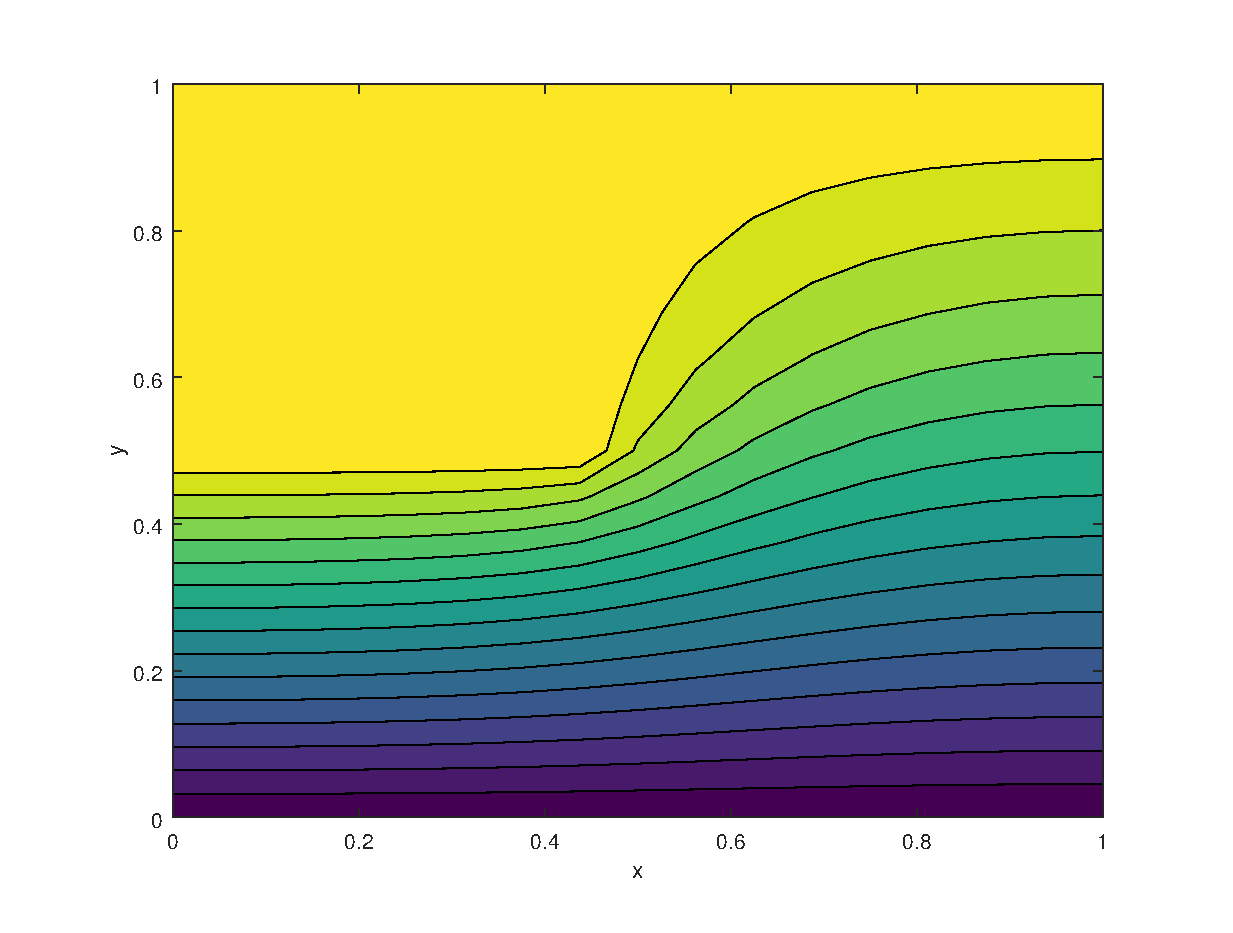
\includegraphics[scale=0.6]{eps/plotPot}
%\end{center}
%\caption[Potentialverlauf eines Kondensators mit Kante]{Potentialverlauf des Kondensators mit Kante.}
%\label{fig:V4.PA4.1}
%\end{figure}

\begin{figure}
	\centering
	\begin{tikzpicture}[scale=1]
		\begin{axis}[
		xlabel={x},
		ylabel={mode},
		%grid=major,
		cycle multi list={color list\nextlist [1 of]mark list},
		legend entries={Grundmode},
		legend style={at={(0.5,-0.2)},anchor=south},
		]
		\addplot table[x=x, y=mode1, col sep=comma] {../csv/modes.csv};
		\addplot+
%		\addplot+ [
%mark=ball,
%mark size=4pt,
%scatter,% enable scatter
%scatter src=rand,% the "color data"
%% configure individual appearances:
%scatter/use mapped color=
%{ball color=mapped color}]
coordinates
{(-0.1,0) (-1,0.1) (0,0) (0.1,0.1) (0.2,0)};

		
		
		\end{axis}
	\end{tikzpicture}
	\caption{asdf}
\end{figure}



\pgfplotstableread[col sep = comma, columns/3/.style={string type}, ignore chars= {(, ),j}] {transfer_fct.csv}\kennlinie %%%%% cannot deal with a 'j' in imaginary part! %%%
%\pgfplotstabletypeset[columns={0,3}, columns/3/.style={string type}] \kennlinie
% erzeugt eine banale Liste

\begin{figure}[hb]
\centering
    \begin{tikzpicture}
\begin{axis}[
		legend entries = {Amplitude},
		legend pos = outer north east,
		]
\addplot[blue, thick] table [ x =0, y index=1] {\kennlinie};

		\addplot [red, mark=o, mark size=5pt]coordinates {(10000000, 8)};
		\addplot coordinates{(20000000, 5)}	;	
		
\end{axis}
\end{tikzpicture}
\caption{Einzelsinus}
\end{figure}

Dies ist ein Versuch, eine Transfer-Function zu plotten mittels tikz:

%\begin{figure}[h!]
%\centering
%    \begin{tikzpicture}
%    \datavisualization [scientific axes=clean, 
%    					visualize as line, 
%    					x axis = {attribute = frequency},
%    					y axis = {attribute = amplitude}]
%    	data [read from file = transfer_fct.csv,
%    			%headline = {frequency, amplitude, phaseshift, complex}
%    			];
%    
    
%\begin{axis}[grid=both, xlabel={$t/T_{\textrm{BB}}$},
%ylabel={$\Usin(t)$},                        ytick={-1,1},
%                        yticklabels={$-\widehat{U}$,$\widehat{U}$},
%                        xtick={-4,-2,0,2,4},
%                        xticklabels={-2,-1,0,1,2}]
%\addplot[blue, thick] table [ x expr={\thisrowno{0}}, y
%expr={\thisrowno{1}}, col sep=semicolon] {csv/transfer_fct.csv};
%\end{axis}
%	\end{tikzpicture}
%\caption{Bsp-Plot einer Transfer-Function H}
%  \label{fig:bsp_transfer}
%\end{figure}


Dies ist ein Versuch, ein Frequenzspektrum zu plotten und Marker an relevanten Punkten zu setzen:




\end{document}